\startchapter{Code Smells}
\label{chapter:smells}

\section{Introduction}


\section{Methodology}
\label{smells:methodology}
In this Section, We explain the methodology we used to address \textbf{RQ-1.2} (How do \cct{} manage programming Idioms and Best Practices?), including how the best practices were sampled (Section~\ref{smells:sampling}), what was the input for copilot (Section~\ref{smells:input}) and how is the suggestion evaluated (Section~\ref{smells:evaluation}). All of the following analysis was carried out using \cop{} extension in Visual Studio Code. We use the most recent stable release of Copilot extension (version number todo) in Visual Studio Code.

\subsection{Sampling Approach}
\label{smells:sampling}
To give the best chance for \cop{} to suggest the optimal way, we sampled the top ten most frequent idioms used in open source projects. So that, \cop{} will have the optimal way more frequently in its training data. However, \cop{} is closed source and we cannot determine if the frequency of code snippet in training data affects \cop{} suggestions in any way. Research by GitHub shows that Copilot can sometimes recite from its training data in ``generic contexts"\footnote{\url{https://github.blog/2021-06-30-github-copilot-research-recitation/}}, which may lead to Licence Infringements shown in Section~\ref{challenges}. Sampling the most frequently used Idioms will also help understand if copilot can recite idioms, which is the ideal behaviour for \cct{}.

\subsection{Study Setup}

\subsubsection{Input to \cop{}}
\label{smells:input}
The input to \cop{} consisted of the idiom title as the first comment to provide context, and the input was restricted to being able to derive the ideal way from the input. This is done to ensure \cop{} is making the decision to suggest the good/bad way in its suggestions. This input style also mimics a novice user, who is unaware of the idioms and useful \cct{} should drive the novice user to use best practices.

\subsubsection{Evaluation}
\label{smells:evaluation}
We considered \cop{} suggested the optimal way if Copilot suggested the best practice in the first suggestion, In this case, we considered \cct{} like \cop{} as productivity tool and user should be saving time as opposed to writing the optimal way without using \cct{}, Scrolling through all the suggestions to deduce the optimal way defeats this purpose. For this reason, We restricted ourselves to first suggestion. However, we do note if the best practice appeared any of the top 10 suggestions currently viewable in \cop{} interface. 

\section{Results}
\subsection{Code Smells}
\label{bp}
A good \AISE{} tool should only suggest code that passes code reviews by humans. We relied on the AirBNB JavaScript coding style guide~\cite{airbnb_code}, a widely used coding style and code review standard. 

The AirBNB JavaScript coding style guide contains a variety of best practices. 
Since, we are testing \cop{} for widely accepted practices and not project specific styling in JavaScript. We chose practices that were closer to design level rather than code level (e.g., logging practices rather than trailing comma use in Javascript).

Using the methodology described in Section~\ref{smells:methodology}, we picked 10 best practices in JavaScript from AirBNB JavaScript coding style guide~\cite{airbnb_code} shown in Table~\ref{tab:all_bp}. \cop{} suggested the recommended way for only one out of the ten standards we tested, i.e, Copilot did not have the recommended way as its top suggestion. Moreover, only 2 out of remaining 9 Best Practices had the Ideal way in \cop{} top 10 suggestions currently viewable. 

% \cop{} performed significantly worse than the Pythonic Idioms we showed in Section~\ref{secidioms}, As \cop{} is closed source, we cannot find the reason behind this but one could argue that lack of data for JavaScript compared to python could be a reason for this behaviour. 

Table~\ref{tab:all_bp} shows the complete list of all the Best Practices we tested on \cop{} from the AirBNB Coding Style guide~\cite{airbnb_code} and the ranking of the Ideal way in \cop{} suggestions (if it exists).

\begin{table}[ht]
    \centering
    \begin{tabular}{|L|c|}
    \hline
         \textbf{Best Practice  Title} & \textbf{\cop{} Suggestion Matched?} \\
         & (out of 10 suggestions) \\
         \hline
         Usage of Object method shorthand & No \\
         \hline
         Array Creating Constructor & 6\textsuperscript{th} \\
         \hline
         Copying Array Contents  & No \\
         \hline
         Logging a Function &  No \\
         \hline
         Exporting a Function & No \\
         \hline
         Sum of Numbers & 9\textsuperscript{th} \\
         \hline
         Accessing Properties & 1\textsuperscript{th} \\
         \hline
         Switch case usage & No \\
         \hline
         Return value from Function with a condition check & No \\
         \hline
         Converting Array-like object to an Array  & No \\
         \hline
    \end{tabular}
    \caption{List of all JavaScript Best Practices tested on \cop{}.}
    \label{tab:all_bp}
\end{table}

Figure~\ref{fig:bp_1} shows the Best Practice for Copying Array Contents, showing user input (i.e., Human Input), the top suggestion by \cop{} and the recommended way suggested by AirBNB JavaScript coding style guide~\cite{airbnb_code}.

All the Best Practices shown in Table~\ref{tab:all_bp} can be found in the \repl{} including the code used as input (i.e., Human Input), the top suggestion by \cop{} and the Ideal Way.

% \begin{tcolorbox}[title=Copying Array Contents,boxsep=.15mm]
%     %https://tex.stackexchange.com/questions/337909/tcolorbox-tcbline-style
% \textbf{Human Input:}
% \begin{lstlisting}[language=JavaScript]
% // copying array contents
% const len = items.length;
% \end{lstlisting}
% \tcbline
% \textbf{Copilot Suggestion:}
% \begin{lstlisting}[language=JavaScript]
% const copy = new Array(len);
% for (let i = 0; i < len; i++) {
% 	  copy[i] = items[i];
% }
% \end{lstlisting}
% \tcbline
% \textbf{Ideal way\footnote{source \cite{airbnb_code}}:}
% \begin{lstlisting}[language=JavaScript]
% const itemsCopy = [...items];
% \end{lstlisting}
% \end{tcolorbox}

%%%%%% TODO: remember to update the screenshot if the source citation is different from the citation in the text %%%%%%
\begin{figure}[hbt!]
    \centering
    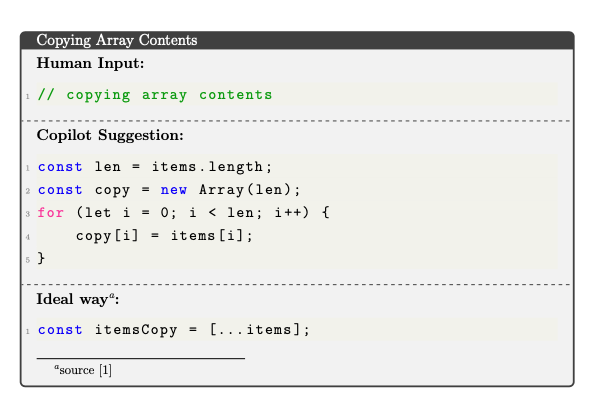
\includegraphics[width=\linewidth]{Figures/bp_1.png}
    \caption{Best Practice for Copying Array Contents amd \cop{} Suggestion.}
    \label{fig:bp_1}
\end{figure}


\section{Chapter Summary}
In summary, we start this chapter by showing the methodology used in addressing textbf{RQ-1} (What are the current boundaries of \cct{}?). 
We first introduced Pythonic idioms and best practices in JavaScript.
We then present our sampling approach for sampling 25 coding scenarios to analyze Copilot code suggestions.
Furthermore, we discussed the input given to Copilot to trigger a code suggestion 
and how the input was restricted to deriving the desired way from the input.
Finally, we described our evaluation approach for Copilot code suggestions.

We sampled 25 Pythonic idioms from Alexandru et al.~\cite{Alexandru2018}, and Farook et al.~\cite{idioms}.
We identified that Copilot did not suggest the idiomatic way as its top suggestion for 23 out of 25 coding scenarios in Python, which addressed \textbf{RQ-1.1} (How do \cct{} manage programming idioms?).
Furthermore, we sampled 25 best practices in JavaScript from the AirBNB JavaScript coding style guide~\cite{airbnb_code}. We identified that Copilot did not suggest the recommended best practice for 22 out of 25 coding scenarios in JavaScript, which addressed \textbf{RQ-1.2} (How do \cct{} manage to manage to suggest non-smelly code?).


% we showed that Copilot struggles to detect and most common idiomatic ways present in public repositories of GitHub and rank them higher than the non-idiomatic ways. The ideal behavior of \cct{} like Copilot in solving this problem is detecting common patterns present in code and rank them higher as the idiomatic ways for a task.
% In the next chapter (chapter~\ref{smells}), we look into how this ideal behavior can cause problems in the case of code smells, where common bad practices present in public repositories of GitHub can make \cct{} like Copilot introduce bad coding practices in its suggestions.

% % \section{Chapter Summary}
% In summary, we start this chapter by showing the methodology used in addressing \textbf{RQ-1.2} (How do \cct{} manage to suggest non-smelly code?). We first introduced the study setup with the input to Copilot and how it was restricted to deriving the best practice from the input and how the suggestions from Copilot were evaluated. We sampled best practices from AirBNB JavaScript coding style guide~\cite{airbnb_code}, and then compared it against Copilot suggestions. Based on results shown in Table~\ref{tab:all_bp}, Copilot struggles to suggest the best practices from widely used coding standards in its suggestions. 

In this chapter, we showed that Copilot struggles to detect and follow coding style guides present in public repositories of GitHub and always suggests code that follows those coding style guides. We also observed that Copilot struggles to detect and most common idiomatic ways present in public repositories of GitHub and rank them higher than the non-idiomatic ways. 
Identifying this delineation could help in urn AI-supported code completion tools such as Copilot into full-fledged AI-supported software engineering tools.
In the next chapter (chapter~\ref{chapter:framework}), we illustrate our taxonomy inspired by autonomous driving levels on the software abstraction hierarchy in \AISE{} and delineate where \cct{} like Copilot currently stands in the taxonomy. 